\section{Ansible I: Simplest Example}\label{ansible-i-simplest-example}

\FILENAME\

\subsection{Prerequisite}\label{prerequisite}

In order to conduct this lesson:

\begin{itemize}
\item
  You can install Ubuntu 16.04 virtual machine on VirtualBox
\item
  You can install software packages via `apt-get' tool in Ubuntu virtual
  host
\item
  You already reserved a virtual cluster (with at least 1 virtual
  machine in it) on some cloud. OR you can use VMs installed in
  VirtualBox instead.
\item
  You set up SSH credentials and can login to your virtual machines.
\end{itemize}

\subsection{What can you do with
Ansible?}\label{what-can-you-do-with-ansible}

Humans do maintenance and configurations on computers. Essentially, we
specify a list of operations and a list of target machines where the
operations apply to. After defining these two critical lists, the
creative works are done, and the rest labour can be automated. And this
is what Ansible is used for.

Let us develop a sample from scratch, based on this paradigm.

\subsection{A sample use case}\label{a-sample-use-case}

In this example, we are going to use Ansible to install Apache server on
our VMs.

\begin{itemize}

\item
  install Ansible tool on your machine first
\end{itemize}

\begin{lstlisting}
$ sudo apt-get update
$ sudo apt-get install ansible
\end{lstlisting}

\begin{itemize}

\item
  prepare a working environment for your Ansible
\end{itemize}

\begin{lstlisting}
$ mkdir}ansible-apache
$ cd ansible-apache
\end{lstlisting}

\begin{itemize}

\item
  next, we are going to create a local configuration file for Ansible.
\end{itemize}

When you execute Ansible within this folder, this local configuration
file is always going to overwrite a system level Ansible configuration.
It is in general beneficial to keep custom configurations locally unless
you absolutely believe it should be applied system wide. Create a file
`ansible.cfg' in this folder, and fill:

\begin{verbatim}
[defaults]
hostfile = hosts
\end{verbatim}

This local configuration file simple tells that the target machines'
names are given in a file named `hosts'

In your assignments, we choose to use \texttt{inventory} instead of
\texttt{ansible.cfg}. More details will be given when we introduce
\texttt{ansible-galaxy} in following chapters. At this moment, getting
yourself familiar with some concepts of configuring the Ansible
environment is good enough.

\begin{itemize}

\item
  specify hosts in the file
\end{itemize}

You should have accesses to all VMs listed in this file as part of our
prerequisites. Create and edit file `hosts':

\begin{verbatim}
[apache]
<server_ip> ansible_ssh_user=<server_username>
\end{verbatim}

The name `apache' in the brackets defines the server group name. We will
use this name to refer to all server items in this group next. Fill in
IP addresses of the virtual machines you launched in your VirtualBox and
fire up these VMs in you VirtualBox.

\begin{itemize}

\item
  compose a playbook
\end{itemize}

A playbook tells Ansible what to do. it uses YAML Markup syntax. Create
and edit a file with a proper name e.g. apache.yml as follow:

\begin{verbatim}
---
- hosts: apache #comment: apache is the group name we just defined
  become: yes #comment: this operation needs privilege access
  tasks:
    - name: install apache2 # text description
      apt: name=apache2 update_cache=yes state=latest
\end{verbatim}

This block defines the target VMs and operations(tasks) need to apply.
you may wonder what `apt' means. here comes the concept of Ansible
modules in next paragraph.

\subsection{The concept of modules}\label{the-concept-of-modules}

`apt' is the module used in our sample playbook. it installs packages on
Ubuntu for us.

Ansible relies on various kinds of modules to fulfil tasks on the remote
servers. These modules are developed for particular tasks and take in
related arguments. For instance, when we use `apt' module, we certainly
need to tell which package we intend to install. That is why we provide
a value for the `name' argument.

\subsection{Run you playbook}\label{run-you-playbook}

In the same folder, execute

\begin{lstlisting}
ansible-playbook apache.yml --ask-sudo-pass
\end{lstlisting}

After a successful run, open a browser and fill in your server IP. you
should se a `It works!' Apache2 Ubuntu default page. Make sure the
security policy on your cloud opens port 80 to let the HTTP traffic go
through.

Ansible playbook can have more complex and fancy structure and syntaxes.
Go explore! this sample is based on:
\url{https://www.digitalocean.com/community/tutorials/how-to-configure-apache-using-ansible-on-ubuntu-14-04}

We are going to offer an advanced Ansible in next chapter.
\section{Ansible II: Roles}\label{ansible-ii-roles}

In this example, we are going to install R package onto your cloud VMs.
R is a useful statistic programing language commonly used in many
scientific and statistics computing projects, maybe also the one you
chose for this class.

In addition to last basic example, we are going to illustrate the
concept of Ansible Roles, install source code through Github, and make
use of variables. These are key features you will find useful in your
project deployments.

We are going to use a top-down fashion in this example. We first start
from a playbook that is already good to go. You can execute this
playbook (do not do it yet) to get R installed in your remote hosts. We
then further complicate this concise playbook by introducing
functionalities to do the same tasks but in different ways. Although
these detours are not necessary in this simply case, it helps you grasp
the power of Ansible and ease your life when they are needed in your
real projects.

\subsection{Prerequisite}\label{prerequisite}

\begin{itemize}

\item
  Finished Ansible Lesson I
\item
  Have VMs reserved on cloud and SSH Key setup
\end{itemize}

\subsection{A completed playbook}\label{a-completed-playbook}

From the earlier example, we already can compose a playbook
`example.yml' that install a software package, for example:

\begin{verbatim}
---
- hosts: R_hosts
  become: yes
  tasks:
    - name: install the R package
      apt: name=r-base update_cache=yes state=latest
\end{verbatim}

the hosts are defined in a file `hosts', which we configured in
`ansible.cfg':

\begin{verbatim}
[R_hosts]
<cloud_server_ip> ansible_ssh_user=<cloud_server_username>
\end{verbatim}

In your assignments, we choose to use \texttt{inventory} instead of
\texttt{ansible.cfg}. More details will be given when we introduce
\texttt{ansible-galaxy} in following chapters. At this moment, getting
yourself familiar with some concepts of configuring the Ansible
environment is good enough.

This should get the installation job done. But we are going to extend it
via new features next.

\subsection{Introducing Roles}\label{introducing-roles}

Role is an important concept used very often in large Ansible projects.
You divide a series of tasks into different groups. Each group
corresponds to certain role of the whole project.

For example, if your project is to deploy a web site, you may need to
install the back end database, the web server that responses HTTP
requests and the web application itself. They are three different roles
and should carry out their own installation and configuration tasks.

Even though we only need to install the R package in this example, we
can still do it by defining a role `r'. Modify your `example.yml' to be:

\begin{verbatim}
---
- hosts: R_hosts

  roles:
    - r
\end{verbatim}

and create directory structure in your top project directory:

\begin{verbatim}
$ mkdir -p roles/r/tasks
$ touch roles/r/tasks/main.yml
\end{verbatim}

edit this `main.yml' to be:

\begin{verbatim}
---
- name: install the R package
  apt: name=r-base update_cache=yes state=latest
  become: yes
\end{verbatim}

You probably already get the point. We take the `tasks' section out of
the one-for-all example.yml and re-organize them into roles. Each role
specified in example.yml should have its own directory under roles/ and
the tasks need be done by this role is listed in a file `tasks/main.yml'
as above.

\subsection{Install source code from
Github}\label{install-source-code-from-github}

Although R can be installed through the OS package manager (apt-get
etc.), the software used in your projects may not. Many research
projects are available by Git instead. Here we are going to show you how
to install packages from their Git repositories. Instead of directly
executing the module `apt', we pretend Ubuntu does not provide this
package and you have to find it on Git. The source code of R can be
found at \url{https://github.com/wch/r-source.git}. We are going to
clone it to a remote VM's hard drive, build the package and install the
binary there.

To do so, we need a few new Ansible modules. You may remember from last
example that Ansible modules assist us to do various kinds of jobs when
fed correct arguments. No surprise, Ansible has a module `git' to take
care of git-related works, and a `command' module to run shell commands.
Let's modify `roles/r/tasks/main.yml' to be:

\begin{verbatim}
---
- name: get R package source
  git:
    repo: https://github.com/wch/r-source.git
    dest: /tmp/R

- name: build and install R
  become: yes
  command: chdir=/tmp/R "{{ item }}"
  with_items:
    - ./configure
    - make
    - make install
\end{verbatim}

The role `r' carries out its two tasks now. One to clone the R source
code into /tmp/R, the other uses a series of shell commands to build and
install the packages.

Note that the commands executed by the second task may not be available
on a fresh VM image. But the point of this example is to show an
alternative way to install packages, so we conveniently assume
conditions are all met.

\subsection{Using variables in a separate
file}\label{using-variables-in-a-separate-file}

We typed several string constants in our Ansible scripts so far. In
general, it is a good practice to give these values names and use them
by referring to their names. This way, you complex Ansible project can
be less error prone. Create a file in the same directory, and name it
`vars.yml':

\begin{verbatim}
---
repository: https://github.com/wch/r-source.git
tmp: /tmp/R
\end{verbatim}

Accordingly, we will update our `example.yml':

\begin{verbatim}
---
- hosts: R_hosts
  vars_files:
    - vars.yml
  roles:
    - r
\end{verbatim}

As shown, we specify a `vars_files' telling the script that the file
`vars.yml' is going to supply variable values, whose keys are denoted by
Double curly brackets like in `roles/r/tasks/main.yml':

\begin{verbatim}
---
- name: get R package source
  git:
    repo: "{{ repository }}"
    dest: "{{ tmp }}"

- name: build and install R
  become: yes
  command: chdir="{{ tmp }}" "{{ item }}"
  with_items:
    - ./configure
    - make
    - make install
\end{verbatim}

\subsection{Summarize}\label{summarize}

Now, just edit the `hosts' file with your target VMs' IP addresses and
execute the playbook.

You should be able to extend the Ansible playbook for your project.
Configuration tools like Ansible are important components to master the
cloud environment. There is much to explore and it's worth it.
\section{Ansible III: Ansible Galaxy}\label{ansible-iii-ansible-galaxy}

By finishing the first two chapters, you should be able to compose
Ansible projects to install, configure or do other maintenance on your
software packages. We introduced the powerful component \texttt{Roles}
in the previous chapters, and emphasized the concepts of modularize and
re-usability. With these preparations, we are ready to start working on
Ansible Galaxy.

Think Ansible Galaxy as of an marketplace, where developers can share
Ansible Roles to complete their system administration tasks. Roles
exchanged in Ansible Galaxy community need to follow common conventions
so that all participants know what to expect. We will illustrate details
in this chapter.

It is good to follow the Ansible Galaxy standard during your development
assignment as much as possible, however, you will submit your
assignments to this class's repository not the global Galaxy community.

\subsection{Ansible Galaxy helloworld}\label{ansible-galaxy-helloworld}

Let us start with a simplest case: We will build an Ansible Galaxy
project. This project will install the Emacs software package on your
localhost as the target host. It is a ``helloworld'' project only meant
to get us familiar with Ansible Galaxy project structures.

\subsubsection{create the directory}\label{create-the-directory}

Setup your submission directory after you clone and rebased with
\url{https://github.com/cloudmesh/sp17-i524}:

\begin{verbatim}
$ git rebase upstream/master
$ ./setup galaxy <your HID>
\end{verbatim}

It will create a folder named after your HID inside directory galaxy/.
Your Galaxy related assignments will be completed and submitted there.
Go ahead and create files \texttt{README.md}, \texttt{playbook.yml},
\texttt{inventory} and a subdirectory \texttt{roles/} then. playbook.yml
is your project playbook. It should perform the Emacs installation task
by executing the corresponding role you will develop in the folder
`roles/'. The only difference is that we will construct the role with
the help of ansible-galaxy this time.

Now, let ansible-galaxy initialize the directory structure for you:

\begin{verbatim}
$ cd roles
$ ansible-galaxy init <to-be-created-role-name>
\end{verbatim}

The naming convention is to concatenate your name and the role name by a
dot. Here is how it looks like:

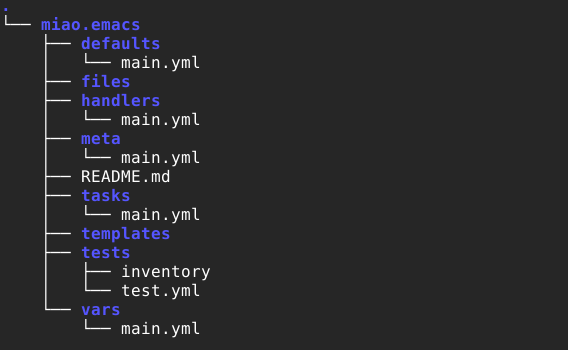
\includegraphics{/images/ansible-galaxy-init-structure.png}

\subsubsection{fill in information}\label{fill-in-information}

Let us fill in information to our project. There are several
\texttt{main.yml} files in different folders, and we will illustrate
their usages.

\begin{description}
\item[defaults and vars:]
These folders should hold variables key-value pairs for your playbook
scripts. We will leave them empty in this example.
\item[files:]
This folder is for files need to be copied to the target hosts. Data
files or configuration files can be specified if needed. We will leave
it empty too.
\item[templates:]
Similar missions to files/, templates is allocated for template files.
Keep empty for a simple Emacs installation.
\item[handlers:]
This is reserved for services running on target hosts. For example, to
restart a service under certain circumstance.
\end{description}

tasks:

\begin{quote}
This file is the actual script for all tasks. You can use the role you
built previously for Emacs installation here:

\begin{verbatim}
---
- name: install Emacs on Ubuntu 16.04
  become: yes
  package: name=emacs state=present
\end{verbatim}
\end{quote}

\begin{description}
\item[meta:]
Provide necessary metadata for our Ansible Galaxy project for shipping:

\begin{verbatim}
---
galaxy_info:
  author: <you name>
  description: emacs installation on Ubuntu 16.04
  license:
    - MIT
  min_ansible_version: 2.0
  platforms:
    - name: Ubuntu
      versions:
        - xenial
  galaxy_tags:
    - development

dependencies: []
\end{verbatim}
\end{description}

\subsubsection{Test it out}\label{test-it-out}

You have your Ansible Galaxy role ready now. To test it as a user, go to
your HID directory and edit the other two files \texttt{inventory} and
\texttt{playbook.yml}, which are already generated for you in directory
\texttt{tests} by the script:

\begin{verbatim}
$ ansible-playbook -i ./hosts playbook.yml
\end{verbatim}

After running this playbook, you should have Emacs installed on
localhost.

\subsection{A Complete Ansible Galaxy
Project}\label{a-complete-ansible-galaxy-project}

We are going to use ansible-galaxy to setup a sample project. This
sample project will:

\begin{itemize}

\item
  use a cloud cluster with multiple VMs
\item
  deploy Apache Spark on this cluster
\item
  install a particular HPC application
\item
  prepare raw data for this cluster to process
\item
  run the experiment and collect results
\end{itemize}
\section{Ansible: Write a Playbooks for
MongoDB}\label{ansible-write-a-playbooks-for-mongodb}

Ansible Playbooks are automated scripts written in YAML data format.
Instead of using manual commands to setup multiple remote machines, you
can utilize Ansible Playbooks to configure your entire systems. YAML
syntax is easy to read and express the data structure of certain Ansible
functions. You simply write some tasks, for example, installing
software, configuring default settings, and starting the software, in a
Ansible Playbook. With a few examples in this section, you will
understand how it works and how to write your own Playbooks.

\begin{description}
\item[There are also several examples of using Ansible
\href{http://docs.ansible.com/playbooks.html}{Playbooks} from the
official site. It covers]
from basic usage of Ansible Playbooks to advanced usage such as applying
patches and updates with different roles and groups.
\end{description}

\subsection{Section: Writing Ansible
Playbook}\label{tutorial-writing-ansible-playbook}

In this section, we are going to write a basic playbook of Ansible
software. Keep in mind that \texttt{Ansible} is a main program and
\texttt{playbook} is a template that you would like to use. You may have
several playbooks in your Ansible.

\subsubsection{First playbook for MongoDB
Installation}\label{first-playbook-for-mongodb-installation}

As a first example, we are going to write a playbook which installs
MongoDB server. It includes the following tasks:

\begin{itemize}

\item
  Import the public key used by the package management system
\item
  Create a list file for MongoDB
\item
  Reload local package database
\item
  Install the MongoDB packages
\item
  Start MongoDB
\end{itemize}

This section is based on the manual installation of MongoDB from the
official site:
\url{http://docs.mongodb.org/manual/tutorial/install-mongodb-on-ubuntu/*}

We also assume that we install MongoDB on Ubuntu 15.10.

\subsubsection{Enabling Root SSH Access}\label{enabling-root-ssh-access}

Some setups of managed nodes may not allow you to log in as root. As
this may be problematic later, let us create a playbook to resolve this.
Create a \texttt{enable-root-access.yaml} file with the following
contents:

\begin{verbatim}
---
- hosts: ansible-test
  remote_user: ubuntu
  tasks:
    - name: Enable root login
      shell: sudo cp ~/.ssh/authorized_keys /root/.ssh/
\end{verbatim}

Explanation:

\begin{itemize}

\item
  \texttt{hosts} specifies the name of a group of machines in the
  inventory
\item
  \texttt{remote_user} specifies the username on the managed nodes to
  log in as
\item
  \texttt{tasks} is a list of tasks to accomplish having a \texttt{name}
  (a description) and modules to execute. In this case we use the
  \texttt{shell} module.
\end{itemize}

We can run this playbook like so:

\begin{verbatim}
$ ansible-playbook -i inventory.txt -c ssh enable-root-access.yaml

PLAY [ansible-test] *********************************************************** 

GATHERING FACTS *************************************************************** 
ok: [10.23.2.105]
ok: [10.23.2.104]

TASK: [Enable root login] ***************************************************** 
changed: [10.23.2.104]
changed: [10.23.2.105]

PLAY RECAP ******************************************************************** 
10.23.2.104                : ok=2    changed=1    unreachable=0    failed=0   
10.23.2.105                : ok=2    changed=1    unreachable=0    failed=0
\end{verbatim}

\subsubsection{Hosts and Users}\label{hosts-and-users}

First step is choosing hosts to install MongoDB and a user account to
run commands (tasks). We start with the following lines in the example
filename of \texttt{mongodb.yaml}:

\begin{verbatim}
---
- hosts: ansible-test
  remote_user: root
  become: yes
\end{verbatim}

In a previous section, we setup two machines with \texttt{ansible-test}
group name. In this section we use two machines for MongoDB
installation. Also, we use \texttt{root} account to complete Ansible
tasks.

\begin{description}
\item[Indentation is important in YAML format. Do not ignore spaces
start]
with in each line.
\end{description}

\subsubsection{Tasks}\label{tasks}

A list of tasks contains commands or configurations to be executed on
remote machines in a sequential order. Each task comes with a
\texttt{name} and a \texttt{module} to run your command or
configuration. You provide a description of your task in \texttt{name}
section and choose a \texttt{module} for your task. There are several
modules that you can use, for example, \texttt{shell} module simply
executes a command without considering a return value. You may use
\texttt{apt} or \texttt{yum} module which is one of the packaging
modules to install software. You can find an entire list of modules
here: \url{http://docs.ansible.com/list_of_all_modules.html}

\subsubsection{\texorpdfstring{Module \texttt{apt\_key}: add repository
keys}{Module apt\_key: add repository keys}}\label{module-apt_key-add-repository-keys}

We need to import the MongoDB public GPG Key. This is going to be a
first task in our playbook.:

\begin{verbatim}
tasks:
  - name: Import the public key used by the package management system
    apt_key: keyserver=hkp://keyserver.ubuntu.com:80 id=7F0CEB10 state=present
\end{verbatim}

\subsubsection{\texorpdfstring{Module \texttt{apt\_repository}: add
repositories}{Module apt\_repository: add repositories}}\label{module-apt_repository-add-repositories}

Next add the MongoDB repository to apt:

\begin{verbatim}
- name: Add MongoDB repository
  apt_repository: repo='deb http://downloads-distro.mongodb.org/repo/ubuntu-upstart dist 10gen' state=present
\end{verbatim}

\subsubsection{\texorpdfstring{Module \texttt{apt}: install
packages}{Module apt: install packages}}\label{module-apt-install-packages}

We use \texttt{apt} module to install \texttt{mongodb-org} package.
\texttt{notify} action is added to start \texttt{mongodb} after the
completion of this task. Use the \texttt{update\_cache=yes} option to
reload the local package database.:

\begin{verbatim}
- name: install mongodb
  apt: pkg=mongodb-org state=latest update_cache=yes
  notify:
  - start mongodb
\end{verbatim}

\subsubsection{\texorpdfstring{Module \texttt{service}: manage
services}{Module service: manage services}}\label{module-service-manage-services}

We use \texttt{handlers} here to start or restart services. It is
similar to \texttt{tasks} but will run only once.:

\begin{verbatim}
handlers:
  - name: start mongodb
    service: name=mongod state=started
\end{verbatim}

\subsubsection{The Full Playbook}\label{the-full-playbook}

Our first playbook looks like this:

\begin{verbatim}
---
- hosts: ansible-test
  remote_user: root
  become: yes
  tasks:
  - name: Import the public key used by the package management system
    apt_key: keyserver=hkp://keyserver.ubuntu.com:80 id=7F0CEB10 state=present
  - name: Add MongoDB repository
    apt_repository: repo='deb http://downloads-distro.mongodb.org/repo/ubuntu-upstart dist 10gen' state=present
  - name: install mongodb
    apt: pkg=mongodb-org state=latest update_cache=yes
    notify:
    - start mongodb
  handlers:
    - name: start mongodb
      service: name=mongod state=started
\end{verbatim}

\subsubsection{Running a Playbook}\label{running-a-playbook}

We use \texttt{ansible-playbook} command to run our playbook:

\begin{verbatim}
$ ansible-playbook -i inventory.txt -c ssh mongodb.yaml

PLAY [ansible-test] *********************************************************** 

GATHERING FACTS *************************************************************** 
ok: [10.23.2.104]
ok: [10.23.2.105]

TASK: [Import the public key used by the package management system] *********** 
changed: [10.23.2.104]
changed: [10.23.2.105]

TASK: [Add MongoDB repository] ************************************************ 
changed: [10.23.2.104]
changed: [10.23.2.105]

TASK: [install mongodb] ******************************************************* 
changed: [10.23.2.104]
changed: [10.23.2.105]

NOTIFIED: [start mongodb] ***************************************************** 
ok: [10.23.2.105]
ok: [10.23.2.104]

PLAY RECAP ******************************************************************** 
10.23.2.104                : ok=5    changed=3    unreachable=0    failed=0   
10.23.2.105                : ok=5    changed=3    unreachable=0    failed=0
\end{verbatim}

If you rerun the playbook, you should see that nothing changed:

\begin{verbatim}
$ ansible-playbook -i inventory.txt -c ssh mongodb.yaml 

PLAY [ansible-test] *********************************************************** 

GATHERING FACTS *************************************************************** 
ok: [10.23.2.105]
ok: [10.23.2.104]

TASK: [Import the public key used by the package management system] *********** 
ok: [10.23.2.104]
ok: [10.23.2.105]

TASK: [Add MongoDB repository] ************************************************ 
ok: [10.23.2.104]
ok: [10.23.2.105]

TASK: [install mongodb] ******************************************************* 
ok: [10.23.2.105]
ok: [10.23.2.104]

PLAY RECAP ******************************************************************** 
10.23.2.104                : ok=4    changed=0    unreachable=0    failed=0   
10.23.2.105                : ok=4    changed=0    unreachable=0    failed=0
\end{verbatim}

\subsubsection{Sanity Check: Test
MongoDB}\label{sanity-check-test-mongodb}

Let's try to run `mongo' to enter mongodb shell.:

\begin{verbatim}
$ ssh ubuntu@$IP
$ mongo
MongoDB shell version: 2.6.9
connecting to: test
Welcome to the MongoDB shell.
For interactive help, type "help".
For more comprehensive documentation, see
        http://docs.mongodb.org/
Questions? Try the support group
        http://groups.google.com/group/mongodb-user
> 
\end{verbatim}

\subsubsection{Terms}\label{terms}

\begin{itemize}

\item
  Module: Ansible library to run or manage services, packages, files or
  commands.
\item
  Handler: A task for notifier.
\item
  Task: Ansible job to run a command, check files, or update
  configurations.
\item
  Playbook: a list of tasks for Ansible nodes. YAML format used.
\item
  YAML: Human readable generic data serialization.
\end{itemize}

\subsubsection{Reference}\label{reference}

The main tutorial from Ansible is here:
\url{http://docs.ansible.com/playbooks_intro.html}

You can also find an index of the ansible modules here:
\url{http://docs.ansible.com/modules_by_category.html}
\section{Ansible Assignment}\label{ansible-assignment}

We have shown a couple of examples of using Ansible tools. Before you
apply it in you final project, we will practice it in this assignment.

\subsection{Requirements}\label{requirements}

\begin{itemize}

\item
  use the \texttt{galaxy} directory in the class assignment repository
\item
  set up the project structure similar to Ansible Galaxy example
\item
  install MongoDB from the package manager (apt in this class)
\item
  configure your MongoDB installation to start the service automatically
\item
  use default port and let it serve local client connections only
\end{itemize}
